\documentclass[10pt]{beamer}

\usetheme{m}
\metroset{progressbar=frametitle}
\setbeamercolor{progress bar}{mLightGreen}

\usepackage{pgfpages}
% \setbeameroption{show notes on second screen}
\usepackage{multimedia}
\usepackage{booktabs}

\usepackage[square]{natbib} % Bibliography, citing: [\citet{storm_nonlinear_2005}]
\usepackage[scale=2]{ccicons}

\usepackage{pgfplots}
\usepgfplotslibrary{dateplot}
\graphicspath{{Figures/}}
\graphicspath{{Videos/}}
\title{Image Analysis on Biopolymer Networks}
\subtitle{Characterization using graphs}
\date{\today}
\author{\textbf{Pablo Hernandez-Cerdan} \emph{\newline \textit{Main Advisor}:} \underline{M.A.K Williams}}
\institute{PhD. Student \newline
    Institute of Fundamental Sciences, Massey University\newline
    MacDiarmid Institute for Advanced Materials and Nanotechnology\newline
    Riddet Institute\newline
    \alert{New Zealand}
}
% \titlegraphic{\hfill
\includegraphics[height=1.5cm]{./logo.pdf}}
\begin{document}

\maketitle

\begin{frame}
  \frametitle{Table of Contents}
  \setbeamertemplate{section in toc}[sections numbered]
  % \tableofcontents[hideallsubsections]
  \tableofcontents[hideallsubsections]
\end{frame}

\section{Intro: Biopolymers in the meso-scale}
\begin{frame}[t]{Motivation: Onset of Strain-Stiffening}
    \citep{storm_nonlinear_2005}
\end{frame}
\begin{frame}[t]{Strain-Stiffening: Validity of Affine Deformation approximation}
    \begin{center} \citep{wilhelm_elasticity_2003} \citep{onck_alternative_2005} \end{center}
    \begin{columns}[T,onlytextwidth]
      \column{0.5\textwidth}
        \textbf{Affine transformations valid at:}
        \begin{itemize}
            \item Stiff Components
            \item Dense Networks
        \end{itemize}
        \textbf{Non-Affine at:}
        \begin{itemize}
            \item Compliant Components
            \item Coarse Networks
        \end{itemize}
      \column{0.5\textwidth}
        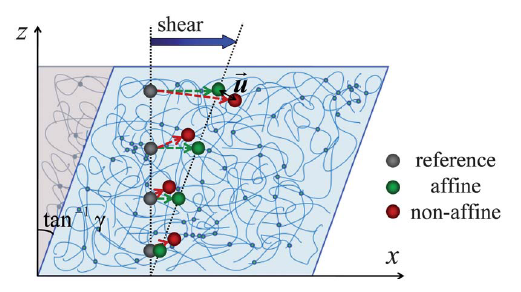
\includegraphics[width=0.9\textwidth]{./Figures/nonaffine.png}
        \newline
        \citep{wen_non-affine_2012,basu_nonaffine_2011}
        \note{
            Difference between affine
            and non-affine deformation of a network under shear. Figure adopted from
            references
        }
        \newline
        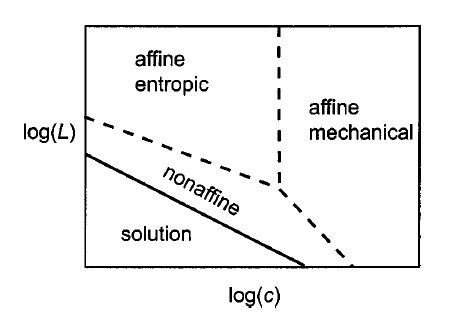
\includegraphics[width=0.9\textwidth]{./Figures/nonaffine-head.png}
        \newline
        \citep{head_mechanical_2005}
        \note{
            Molecular weight (L) and concentration (c). The solid line represents
            the rigidity percolation transition, where rigidity first appears at
            macroscopic level
        }
    \end{columns}
\end{frame}
\begin{frame}
  \frametitle{Goals and research questions}
  \begin{itemize}
      \item Biopolymer gels properties are known to rely heavily on its single-chain components, but also on the way they are linked and interconnected to each other.
      \item Going beyond the isotropic vision of connectivity for biopolymer gels, we want to characterize the architecture of the filaments using images from different microscopy techniques depending on the scale of the biopolymer.
      \item How different architectures do influent the mechanical properties? Are completely different biopolymers sharing universal properties in their connectivity?
  \end{itemize}
\end{frame}
\begin{frame}
    %[allowframbreaks]
    \frametitle{Generating Software Tools}
    \centering
    \movie[height=0.75\textheight, width=\textwidth, poster, autostart, loop, showcontrols]{}{Videos/softwareShort.mp4}

    \note
    {
        Instead of using a one time solution, I am interested in provide computational, user friendly tools for others to use.\newline
        This has driven me to the software development side
    }

\end{frame}
\begin{frame}
  \frametitle{Connectivity matters}

\end{frame}
\begin{frame}
    \frametitle{Polymer Networks: Strain Stiffen}
    \begin{itemize}
        \item \cite{Storm}, strain stiffening arises from non linearity of single chains.
            Under the assumption that the network is isotropic and homogeneus.
            What happen when the network is anisotropic, or it is partially oriented.
        \item  \cite{hola}, at the same time an alternative explanation of strain stiffening arised from
    network connectivity and relative orientation of the fibers.
    \end{itemize}
\end{frame}
\begin{frame}
    \frametitle{The limit of the isotropic approximation}
    \begin{itemize}
        \item The power law behaviour has derived from universal slope of 1 \cite{mackintosh_bill} to \textbf{surprisingly(?)} a slope of  3/2. We think that this data require a further explanation beyond the assumption that collagen is somehow an exception in that universality claimed years ago.
        \item The shift to strain stiffening, or the beginning of a nematic phase of partially oriented fibers, might depend on architecture.
    \end{itemize}
\end{frame}
\begin{frame}
    \frametitle{Steps to characterize the network}
\begin{itemize}
    \item Gathering the images. Microscopy.
    \item Image analysis. Skeletonization.
    \item Characterize the image. Graph approach.
    \note
    {
        Grab the structure of a diluted enough network to be suceptible of the graph approach.
        If it is too dense, probably the study of porosity would be more suitable
    }
\end{itemize}
\end{frame}

\section{Gathering structure data: Experiments.}

\begin{frame}
    \frametitle{Microscopy: Confocal}
\end{frame}
\begin{frame}
    \frametitle{Microscopy: TEM}
\end{frame}
\begin{frame}
    \frametitle{Scattering: SAXS}
\end{frame}
\begin{frame}
  \frametitle{Comparisson of techniques.}
  \begin{columns}[T,onlytextwidth]
    \column{0.33\textwidth}
      Confocal
      \begin{itemize}
        \item Milk \item Eggs \item Potatos
      \end{itemize}

    \column{0.33\textwidth}
      TEM
      \begin{enumerate}
        \item First, \item Second and \item Last.
      \end{enumerate}

    \column{0.33\textwidth}
      SAXS
      \begin{description}
        \item[PowerPoint] Meeh. \item[Beamer] Yeeeha.
      \end{description}
  \end{columns}
\end{frame}

\section{Image Analysis}

% \begin{frame}{Lists}
%   \begin{columns}[T,onlytextwidth]
%     \column{0.33\textwidth}
%       Items
%       \begin{itemize}
%         \item Milk \item Eggs \item Potatos
%       \end{itemize}

%     \column{0.33\textwidth}
%       Enumerations
%       \begin{enumerate}
%         \item First, \item Second and \item Last.
%       \end{enumerate}

%     \column{0.33\textwidth}
%       Descriptions
%       \begin{description}
%         \item[PowerPoint] Meeh. \item[Beamer] Yeeeha.
%       \end{description}
%   \end{columns}
% \end{frame}
% \begin{frame}{Animation}
%   \begin{itemize}[<+- | alert@+>]
%     \item \alert<4>{This is\only<4>{ really} important}
%     \item Now this
%     \item And now this
%   \end{itemize}
% \end{frame}
% \begin{frame}{Figures}
%   \begin{figure}
%     \newcounter{density}
%     \setcounter{density}{20}
%     \begin{tikzpicture}
%       \def\couleur{alerted text.fg}
%       \path[coordinate] (0,0)  coordinate(A)
%                   ++( 90:5cm) coordinate(B)
%                   ++(0:5cm) coordinate(C)
%                   ++(-90:5cm) coordinate(D);
%       \draw[fill=\couleur!\thedensity] (A) -- (B) -- (C) --(D) -- cycle;
%       \foreach \x in {1,...,40}{%
%           \pgfmathsetcounter{density}{\thedensity+20}
%           \setcounter{density}{\thedensity}
%           \path[coordinate] coordinate(X) at (A){};
%           \path[coordinate] (A) -- (B) coordinate[pos=.10](A)
%                               -- (C) coordinate[pos=.10](B)
%                               -- (D) coordinate[pos=.10](C)
%                               -- (X) coordinate[pos=.10](D);
%           \draw[fill=\couleur!\thedensity] (A)--(B)--(C)-- (D) -- cycle;
%       }
%     \end{tikzpicture}
%     \caption{Rotated square from
%     \href{http://www.texample.net/tikz/examples/rotated-polygons/}{texample.net}.}
%   \end{figure}
% \end{frame}
% \begin{frame}{Tables}
%   \begin{table}
%     \caption{Largest cities in the world (source: Wikipedia)}
%     \begin{tabular}{lr}
%       \toprule
%       City & Population\\
%       \midrule
%       Mexico City & 20,116,842\\
%       Shanghai & 19,210,000\\
%       Peking & 15,796,450\\
%       Istanbul & 14,160,467\\
%       \bottomrule
%     \end{tabular}
%   \end{table}
% \end{frame}
% \begin{frame}{Blocks}
%   Three different block environments are pre-defined and may be styled with an
%   optional background color.

%   \begin{columns}[T,onlytextwidth]
%     \column{0.5\textwidth}
%       \begin{block}{Default}
%         Block content.
%       \end{block}

%       \begin{alertblock}{Alert}
%         Block content.
%       \end{alertblock}

%       \begin{exampleblock}{Example}
%         Block content.
%       \end{exampleblock}

%     \column{0.5\textwidth}

%       \metroset{block=fill}

%       \begin{block}{Default}
%         Block content.
%       \end{block}

%       \begin{alertblock}{Alert}
%         Block content.
%       \end{alertblock}

%       \begin{exampleblock}{Example}
%         Block content.
%       \end{exampleblock}

%   \end{columns}
% \end{frame}
% \begin{frame}{Math}
%   \begin{equation*}
%     e = \lim_{n\to \infty} \left(1 + \frac{1}{n}\right)^n
%   \end{equation*}
% \end{frame}
% \begin{frame}{Line plots}
%   \begin{figure}
%     \begin{tikzpicture}
%       \begin{axis}[
%         mlineplot,
%         width=0.9\textwidth,
%         height=6cm,
%       ]

%         \addplot {sin(deg(x))};
%         \addplot+[samples=100] {sin(deg(2*x))};

%       \end{axis}
%     \end{tikzpicture}
%   \end{figure}
% \end{frame}
% \begin{frame}{Bar charts}
%   \begin{figure}
%     \begin{tikzpicture}
%       \begin{axis}[
%         mbarplot,
%         xlabel={Foo},
%         ylabel={Bar},
%         width=0.9\textwidth,
%         height=6cm,
%       ]

%       \addplot plot coordinates {(1, 20) (2, 25) (3, 22.4) (4, 12.4)};
%       \addplot plot coordinates {(1, 18) (2, 24) (3, 23.5) (4, 13.2)};
%       \addplot plot coordinates {(1, 10) (2, 19) (3, 25) (4, 15.2)};

%       \legend{lorem, ipsum, dolor}

%       \end{axis}
%     \end{tikzpicture}
%   \end{figure}
% \end{frame}
\begin{frame}{References}
  Some references to showcase [allowframebreaks] \cite{knuth92,ConcreteMath,Simpson,Er01,greenwade93}
\end{frame}


\section{Graph Characterization}

\section{Conclusion}

\begin{frame}{Summary}

  Get the source of this theme and the demo presentation from

  \begin{center}\url{github.com/matze/mtheme}\end{center}

  The theme \emph{itself} is licensed under a
  \href{http://creativecommons.org/licenses/by-sa/4.0/}{Creative Commons
  Attribution-ShareAlike 4.0 International License}.

  \begin{center}\ccbysa\end{center}

\end{frame}

\plain{Questions?}

\begin{frame}[allowframebreaks]

  \frametitle{References}

  \bibliography{leipzig2015}
  \bibliographystyle{plainnat}

\end{frame}

\end{document}
